\chapter{Case study: slow client}\label{ch:case_study}

\section{Descrizione}\label{s:descrizione}

Il \textit{case study} prevede l'analisi delle prestazioni di un \textit{server} che accetta due tipi di richieste:
\begin{itemize}
    \item \textbf{Richieste lente}\footnotemark{}: all'interno di un'applicazione reale, una richiesta lenta può rappresentare operazioni \textit{I/O bound} (connessioni ad un database, richieste a servizi esterni, operazioni su disco etc.) o \textit{CPU bound} (operazioni di crittografia, calcoli matematici avanzati etc.);
    \item \textbf{Richieste veloci}\footnotemark[\value{footnote}]: sono operazioni leggere che richiedono pochi passaggi in memoria (aggiornamento di variabili locali, lettura da cache, operazioni matematiche semplici etc.)
\end{itemize}

\footnotetext{In questo contesto, per "velocità" si intende il tempo medio di esecuzione di un processo ed è relativo alle richieste stesse. Per richieste di velocità diverse, infatti, si indicano processi i cui tempi di esecuzione viaggiano su ordini di grandezza differenti.}

Se non gestiti correttamente, i due flussi in ingresso possono condurre il sistema ad un situazione di \textit{trashing} in cui entrambe le classi di traffico soffrono di \textit{performance} degradate. Infatti, con riferimento ai parametri descritti in \cref{s:mm1}, la gestione inefficiente delle richieste lente comporta un aumento del numero medio di processi nel sistema, con conseguente aumento del tempo medio di risposta (e tempo di attesa) sia delle richieste lente, ma anche di quelle veloci\cite{644616}.\\

Lo scopo dell'analisi è quello di fornire una comparazione delle prestazioni del server utilizzando due algoritmi di \textit{scheduling} differenti: FCFS (\textit{first come first served}) e DRR (\textit{deficit round robin}), In particolare, l'attenzione sarà posta su come variano le \textit{performance} quando, utilizzando DRR, viene data maggiore priorità alle richieste veloci.

\section{Esperimento}\label{ch:esperimento}

L'esperimento prevede la creazione di un'architettura client-server. Il \textit{client} si occupa di orchestrare l'invio di \textit{workload} al server che risponde ad ogni richiesta con le informazioni utili all'analisi delle prestazioni.\\
Al fine di evidenziare il fenomeno di degradazione delle performance, l'esperimento sarà condotto utilizzando connessioni TCP in quanto ciascuna connessione richiede l'allocazione di risorse predicibili che producono delle variazioni significative nei parametri misurati.

\subsection{Metodologie utilizzate}\label{s:metodologie}
In questa sezione, sono descritte le tecniche e le tecnologie utilizzate per condurre l'esperimento.

\subsubsection{Hardware}
Client e server sono due macchine virtuali installate in server diversi con le specifiche tecniche descritte in \cref{tab:server_spec} e \cref{tab:client_spec}.

\begin{table}
    \centering
    \begin{tabular}{|p{2.5cm}||p{9cm}| }
        \hline
         RAM& 1GB, ECC DIMM\\
         \hline
         \hline
         CPU& 1vCPU, 2GHz\\
         \hline
         \hline
         Network& Virtual adapter con driver VirtIO\\
         \hline
         \hline
         OS& Debian 11, kernel 5.10.0-16-amd64\\
         \hline
    \end{tabular}
    \caption{Specifiche tecniche macchina server.}
    \label{tab:server_spec}
\end{table}

\begin{table}
    \centering
    \begin{tabular}{|p{2.5cm}||p{9cm}| }
        \hline
         RAM& 2GB, ECC DIMM\\
         \hline
         \hline
         CPU& 1vCPU, 2.2GHz\\
         \hline
         \hline
         Network& Virtual adapter con driver VirtIO\\
         \hline
         \hline
         OS& Ubuntu 20.04 LTS, kernel 5.4.0-96-generic\\
         \hline
    \end{tabular}
    \caption{Specifiche tecniche macchina client.}
    \label{tab:client_spec}
\end{table}

\subsubsection{Go (Golang)}
Go è un linguaggio di programmazione compilato \textit{general purpose} creato in Google nel 2009. Il linguaggio è dotato di un \textit{runtime} multiprocessore \textit{m:n}\footnote{Con questa notazione si indica che il runtime è in grado di gestire m \textit{task} su n processi di sistema operativo. In generale, Go esegue lo \textit{scheduling} dei \textit{task} effettuando il \textit{multiplexing} su un numero di processi uguale a quello dei processori fisici rilevati.} e di \textit{garbage collector}. Go offre un'implementazione nativa di \textit{Communication Sequential Process} (\textit{CSP}) che, insieme alle \textit{goroutine}, lo rende adatto all'implementazione di sistemi concorrenti e ad eventi. Una \textit{goroutine} è l'implementazione di un \textit{thread} che esegue nello spazio utente\footnote{In altre tecnologie, possono essere indicati con \textit{coroutine}, \textit{light thread} o \textit{green thread}.}. In particolare, la realizzazione dei CSP avviene attraverso strutture dette \textit{channel} che si occupano di far comunicare \textit{goroutine} separate, garantendo una consegna ordinata dei messaggi.
Inoltre, il linguaggio mette a disposizione un'implementazione del costrutto \textit{select} che, analogamente alla \textit{system call} \textit{Linux}, consente di monitorare più \textit{channel} bloccandosi fino a quando \textbf{almeno} uno di questi non riceve un messaggio\footnote{In Go, è disponibile una variante non bloccante di questo costrutto mediante il ramo \textit{default} che viene eseguito immediatamente se nessun \textit{channel} è pronto.}.

\subsubsection{Python}
Python è un linguaggio di programmazione interpretato \textit{general purpose}. In questo elaborato, viene utilizzato principalmente per effettuare l'analisi dei risultati dell'esperimento (\cref{s:risultati}). In particolare, con l'utilizzo delle librerie \textit{pandas}\cite{reback2020pandas} e \textit{matplotlib}\cite{Hunter:2007} vengono manipolati i CSV generati, create delle tabelle \textit{pivot} che mettono in relazione i due algoritmi di \textit{scheduling}, estratte le informazioni desiderate e rappresentate graficamente. Nello specifico, nell'ottica della riproducibilità dell'analisi dei risultati, è stato creato un Jupyter notebook\cite{Giuseppe_tesi_2022}.\\
Inoltre, Python viene utilizzato per la creazione del \textit{workload} descritta in \cref{s:workload}.

\subsection{Creazione del workload}\label{s:workload}
Il \textit{workload} è l'insieme di attività da effettuare sul server e viene generato dallo script in \textit{workload.py}\cite{Giuseppe_tesi_2022}, salvato in un file JSON e passato in ingresso al programma \textit{client}\cite{Giuseppe_tesi_2022} che si occupa di effettuare l'attività di \textit{benchmark} e salvare i risultati su un file CSV. Le singole attività sono caratterizzate dalle seguenti proprietà:
\begin{itemize}
    \item \textbf{slow\_rate}: numero di richieste lente da inviare al secondo. In base al numero di partenza, di fine e un incremento, lo script genera un insieme di valori con incremento fisso;
    \item \textbf{fast\_rate}: numero di richieste veloci da inviare al secondo. L'intervallo generato è analogo a quello delle richieste lente;
    \item \textbf{slow\_percent}: percentuale di richieste lente da inviare in relazione al numero di richieste totali. Analogamente ai precedenti insiemi, anche questo intervallo varia secondo una progressione ad incremento fisso;
\end{itemize}

Una volta creati gli intervalli dei parametri, il \textit{workload} viene generato facendo il prodotto cartesiano degli insiemi ottenuti. 

\section{Implementazione}

Il funzionamento generale dell'esperimento è riassunto in \cref{fig:general}.

\begin{figure}
  \centering
  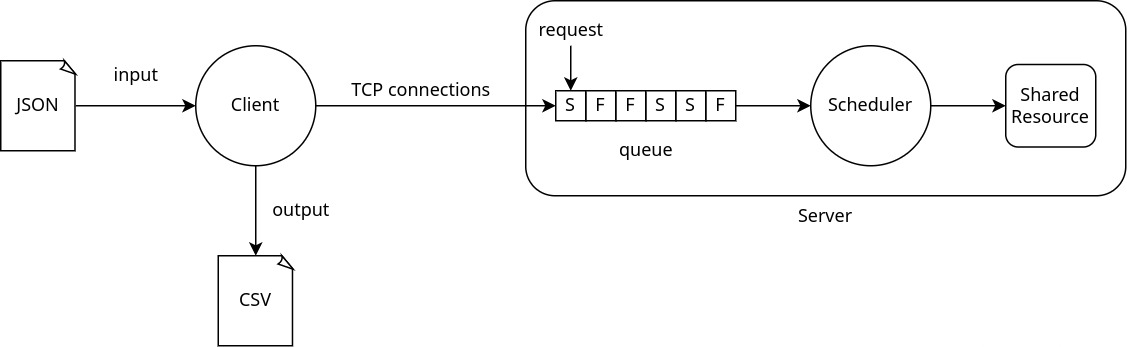
\includegraphics[width=\textwidth]{img/arch/tesi-generale (1).jpg}
  \caption{Schema di funzionamento generale dell'esperimento.}
  \label{fig:general}
\end{figure}

\subsection{Client}
Il client\cite{Giuseppe_tesi_2022} legge da un file una lista di workload e li invia al server. In particolare, il \textit{client} genera una \textit{goroutine} separata per ogni richiesta con una temporizzazione che segue una distribuzione esponenziale (\ref{s:limiti}) e salva le metriche raccolte in un file CSV. Per avere un esperimento più realistico e rendere indipendenti le richieste, il \textit{client} aprirà una nuova connessione per ogni richiesta\footnote{In ogni connessione viene inviata una sola richiesta} e non adotterà alcuna tecnica di \textit{caching} e/o \textit{pooling} delle connessioni che andrebbero a falsare i valori di \textit{round trip time} (RTT, \cref{s:dati}) in quanto verrebbe saltato l'\textit{handshaking} delle connessioni TCP.

\subsection{Server}
Il server\cite{Giuseppe_tesi_2022} si mette in ascolto di connessioni TCP e utilizza una \textit{goroutine} separata per lo \textit{scheduling} delle richieste. L'implementazione dello \textit{scheduling} avviene attraverso il \textit{multiplexing} dei flussi in ingresso in un unico flusso d'uscita, mediante \textit{channel} (\cref{fig:fcfs} e \cref{fig:drr}). Ad ogni richiesta, codificata come un \textit{uint32}\footnote{Il \textit{client} invia $0$ per una richiesta lenta e $1$ per una richiesta veloce}, il server risponde con un documento JSON in cui sono presenti le metriche (\cref{s:dati}) per l'analisi finale.
Al fine di limitare l'ottimizzazione dello \textit{scheduler} interno di Go e di avere risultati realistici, è stato deciso di utilizzare un server con un solo processore fisico (\cref{s:limiti}). L'implementazione\cite{drr_impl} dello \textit{scheduler} DRR è basata sull'algoritmo descritto in \cref{s:drr}.

\begin{figure}
  \centering
  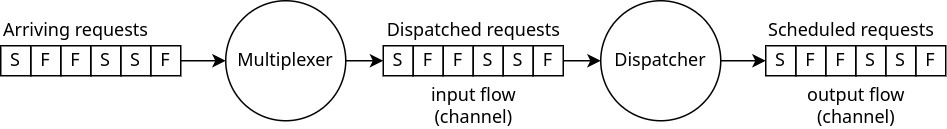
\includegraphics[width=\textwidth]{img/arch/tesi-fcfs.jpg}
  \caption{Implementazione \textit{scheduler} FCFS.}
  \label{fig:fcfs}
\end{figure}

\begin{figure}
  \centering
  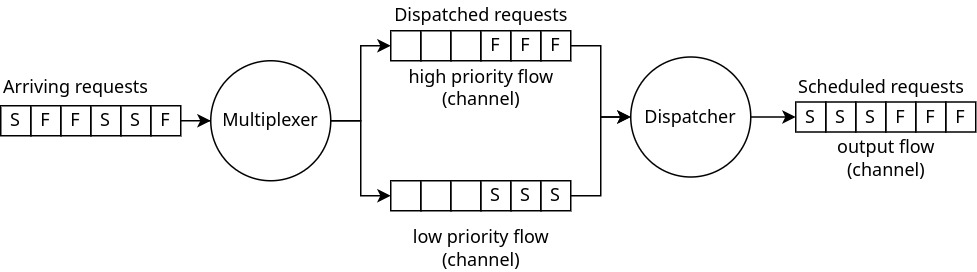
\includegraphics[width=\textwidth]{img/arch/tesi-drr.jpg}
  \caption{Implementazione \textit{scheduler} DRR.}
  \label{fig:drr}
\end{figure}

\section{Raccolta dati}\label{s:dati}

Come accennato in precedenza, per ogni richiesta, il server costruisce una risposta in JSON con i seguenti campi:
\begin{itemize}
    \item \textbf{Istante di accettazione ($I_a$)}: per ogni connessione accettata, il server crea una nuova \textit{goroutine} e, dalla connessione con il client, legge un \textit{uint32} e marca la richiesta come accettata;
    \item \textbf{Istante inizio di esecuzione ($I_e$)}: dopo aver letto il tipo di richiesta, il server ne effettua lo \textit{scheduling}. Quando la richiesta viene schedulata e arriva alla \textit{goroutine} per l'accesso alla risorsa condivisa, la richiesta viene marcata come in esecuzione;
    \item \textbf{Istante di fine esecuzione ($I_f$)}: dopo aver servito la richiesta, viene segnato il tempo di fine esecuzione;
    \item \textbf{Memoria allocata}: insieme al tempo di fine esecuzione viene segnata anche la memoria allocata del sistema al programma server\footnote{Il dato raccolto viene fornito direttamente dal \textit{runtime} e include tutta la memoria allocata dal sistema operativo, insieme allo \textit{stack} e all'\textit{heap} delle singole \textit{goroutine}}.
    \item \textbf{Utilizzazione del processore ($\rho$)}: unitamente alla memoria allocata, nella risposta viene inviato anche l'utilizzazione del processore; 
    \item \textbf{Numero di processi nel sistema ($\overline{K}$)}: assegnando una \textit{goroutine} per ogni connessione ed effettuando esattamente una richiesta per client, il numero di richieste nel sistema corrisponde al numero di \textit{goroutine} escluse quelle già in esecuzione;
\end{itemize}

Con le metriche appena descritte, il \textit{client} calcola le seguenti statistiche:
\begin{itemize}
    \item \textbf{Tempo di residenza medio} ($T_r$): tempo speso dalla richiesta all'interno del sistema. Viene calcolato con $I_f-I_a$;
    \item \textbf{Tempo di attesa medio} ($T_w$): tempo speso dalla richiesta in coda prima di essere servita. Viene calcolato con $I_e - I_a$;
\end{itemize}

Per ogni \textit{workload}, il \textit{client} calcola il valore medio di tutte statistiche illustrate.

\section{Limiti}\label{s:limiti}

\subsection{Misura degli istanti temporali}
Go utilizza uno scheduler \textit{fair} per le sue \textit{goroutine} e, in caso di \textit{system call}, il runtime potrebbe ottimizzare l'operazione con un \textit{context switch}. La presenza di una sola CPU all'interno del server rende possibile un confronto alla pari con altri \textit{runtime} \textit{single-threaded}. 

\subsection{Misurazione utilizzazione del processore}
La misurazione della percentuale di carico della CPU è un'operazione che dipende strettamente dal sistema operativo utilizzato. In questo elaborato, per utilizzazione del processore viene utilizzato il valore medio calcolato nell'ultimo minuto. In particolare, utilizzando un sistema operativo \textit{Linux-based}, questo valore viene letto dal file virtuale \textit{/proc/stat}.

\subsection{Generazione temporizzata degli eventi}
L'implementazione utilizzata per la generazione degli eventi utilizza la funzione \textit{time.After(d time.Duration)}.\\
Quest'approccio presenta due limiti: il tipo \textit{time.Duration} esprime gli intervalli temporali con una precisione del nanosecondo (quindi per \textit{workload} con \textit{rate} molto alti, la risoluzione potrebbe non bastare)\footnote{In Go, il tipo \textit{time.Duration} è un alias per \textit{int64}.}; mentre la funzione \textit{time.After} consegna un messaggio attraverso un \textit{channel} dedicato che non assicura la immediata schedulazione della \textit{goroutine}, ma solo che sia trascorso \textbf{almeno} l'intervallo espresso nel parametro di ingresso.

\section{Risultati}\label{s:risultati}

I risultati presentati di seguito sono stati ottenuti applicando il \textit{workload} descritto in \cref{tab:workload} effettuando $10000$ richieste per blocco. Inoltre, il server serve una richiesta lenta sospendendo l'esecuzione della \textit{goroutine} per un millisecondo.

\begin{table}
    \centering
    \begin{tabular}{|p{3cm}||p{3cm}||p{3cm}||p{3cm}| }
        \hline
        Parametro& Inizio& Fine& Incremento\\
        \hline
         Slow Load & 10 (\%)& 70 (\%)& 20\\
         \hline
         \hline
         Slow rate& 1000 (rps)& 5000 (rps)& 1000\\
         \hline
         \hline
         Fast rate& 1000 (rps)& 5000 (rps)& 1000\\
         \hline
         \hline
    \end{tabular}
    \caption{Parametri utilizzati per generare il \textit{workload}.}
    \label{tab:workload}
\end{table}

\subsection{Analisi richieste lente}
Come anticipato in \cref{s:scheduling}, l'applicazione di un algoritmo a priorità può portare alla \textit{starvation} dei processi a bassa priorità. Infatti, come mostrato in \cref{fig:slow_byslow}, il tempo medio di attesa delle richieste lente è più basso con l'algoritmo FCFS, ma si noti che aumentando la percentuale di carico, le due strategie di \textit{scheduling} tengono a comportarsi allo stesso modo.

\begin{figure}
  \centering
  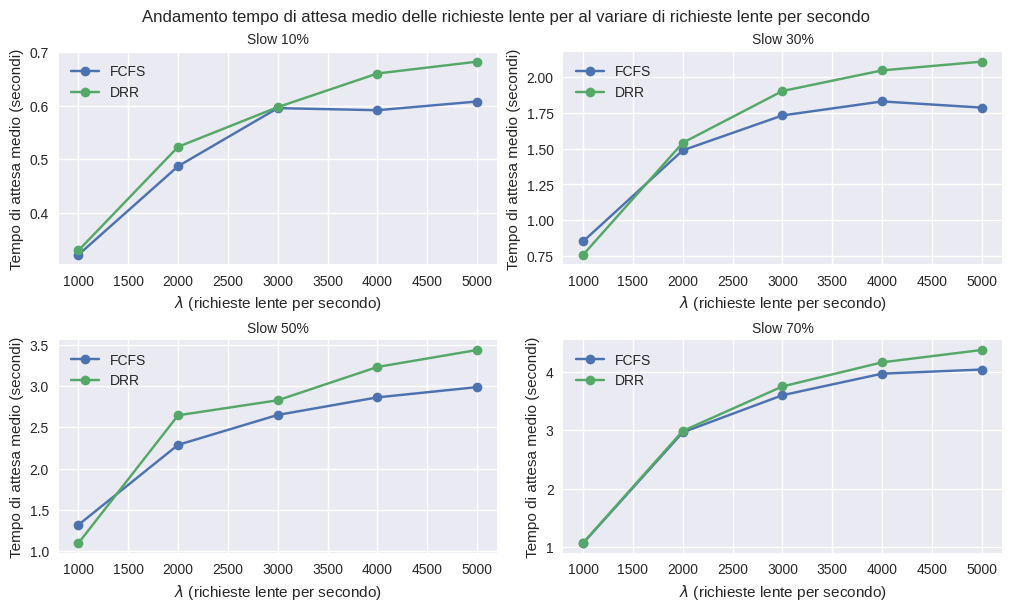
\includegraphics[width=\textwidth]{img/results/slow_wt_byslow.png}
  \caption{Andamento tempo medio di attesa delle richieste lente con variazione del numero di richieste lente per secondo.}
  \label{fig:slow_byslow}
\end{figure}

Inoltre, si noti come facendo variare le richieste veloci, con l'algoritmo DRR, il tempo di attesa delle richieste lente può aumentare del $27\%$ rispetto alla politica FCFS, come mostrato in \cref{fig:slow_byfast}.

\begin{figure}
  \centering
  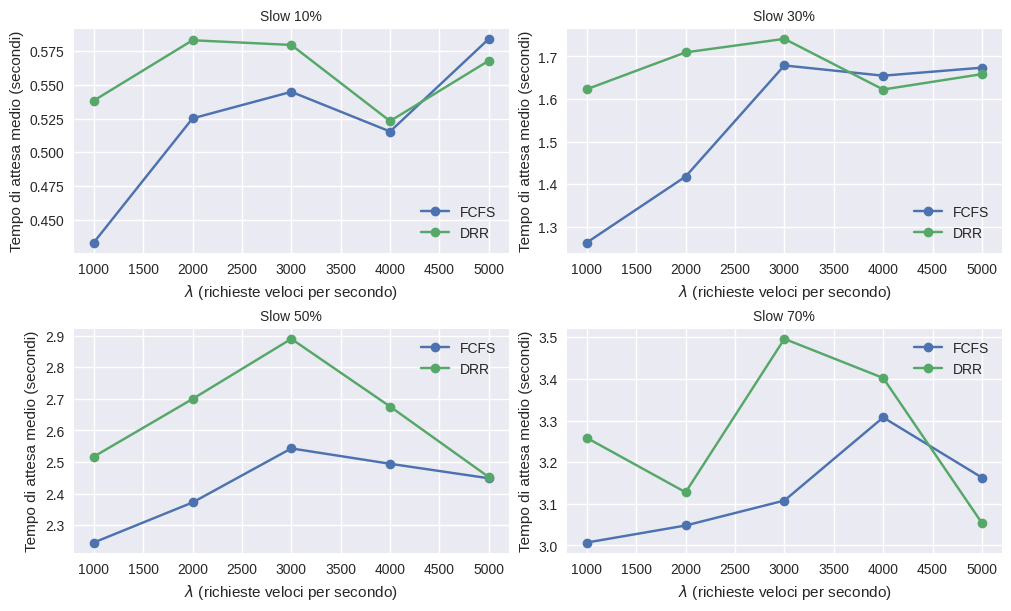
\includegraphics[width=\textwidth]{img/results/slow_wt_byfast.png}
  \caption{Andamento tempo medio di attesa delle richieste lente con variazione del numero di richieste veloci per secondo.}
  \label{fig:slow_byfast}
\end{figure}

\subsection{Analisi richieste veloci}\label{s:fast_an}
Dare una maggiore priorità alle richieste veloci, porta ad un miglioramento generale alle prestazioni del server (\cref{fig:fast_byslow}). Infatti, si noti come ad una crescita pseudo-lineare del tempo di attesa con FCFS, corrisponde un andamento quasi costante con DRR. In particolare, quando il server ha poche richieste lente (\textit{slow=10\%}), DRR risulta sconveniente, ma all'aumentare della frequenza di arrivo si registra un miglioramento dei tempi di attesa di circa il $75\%$; questo miglioramento viene mantenuto anche nel caso in cui il numero di richieste lente è uguale a quelle veloci. Inoltre, il basso tempo di attesa delle richieste veloci contribuisce come illustrato in \cref{s:jobs} a una maggiore capacità del server.

\begin{figure}
  \centering
  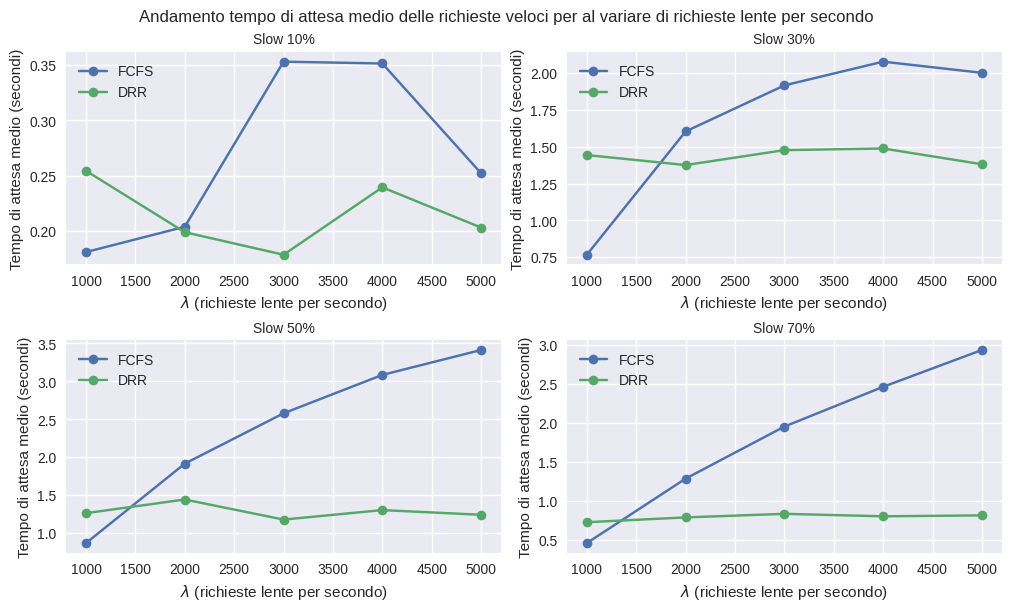
\includegraphics[width=\textwidth]{img/results/fast_by_slow.png}
  \caption{Andamento tempo medio di attesa delle richieste veloci con variazione del numero di richieste lente per secondo.}
  \label{fig:fast_byslow}
\end{figure}

Analogamente, al caso delle richieste lente, osservando come variano i tempi di risposta rispetto alla frequenza delle richieste veloci si evince che i due algoritmi si comportano in modo simile (\cref{fig:fast_byfast}).

\begin{figure}
  \centering
  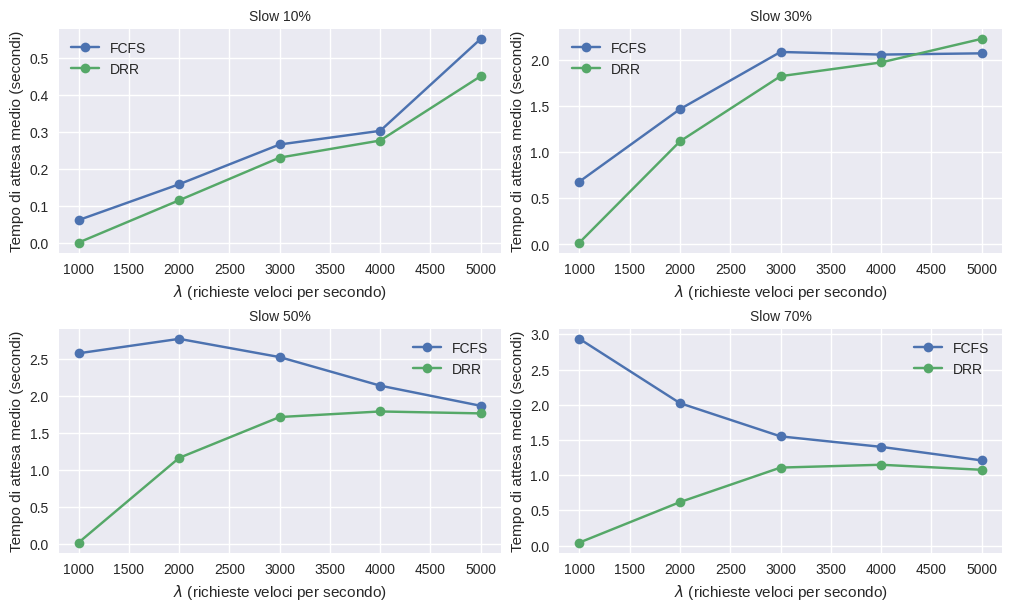
\includegraphics[width=\textwidth]{img/results/fast_byfast.png}
  \caption{Andamento tempo medio di attesa delle richieste veloci con variazione del numero di richieste veloci per secondo.}
  \label{fig:fast_byfast}
\end{figure}

\subsection{Numero di processi nel sistema}\label{s:jobs}
Dall'analisi effettuata in \cref{s:fast_an}, è immediato ricavare che, utilizzando l'algoritmo DRR, il numero di richieste nel sistema si abbassa quando cresce il numero di richieste veloci in quanto vengono servite con priorità maggiore, come mostrato in \cref{fig:jobs}. In particolare, si noti come entrambi gli algoritmi presentano un andamento pseudo-lineare, ma l'algoritmo DRR mostra, anche in presenza di poche richieste veloci (\textit{slow=70\%}), una retta a pendenza minore.


\begin{figure}
  \centering
  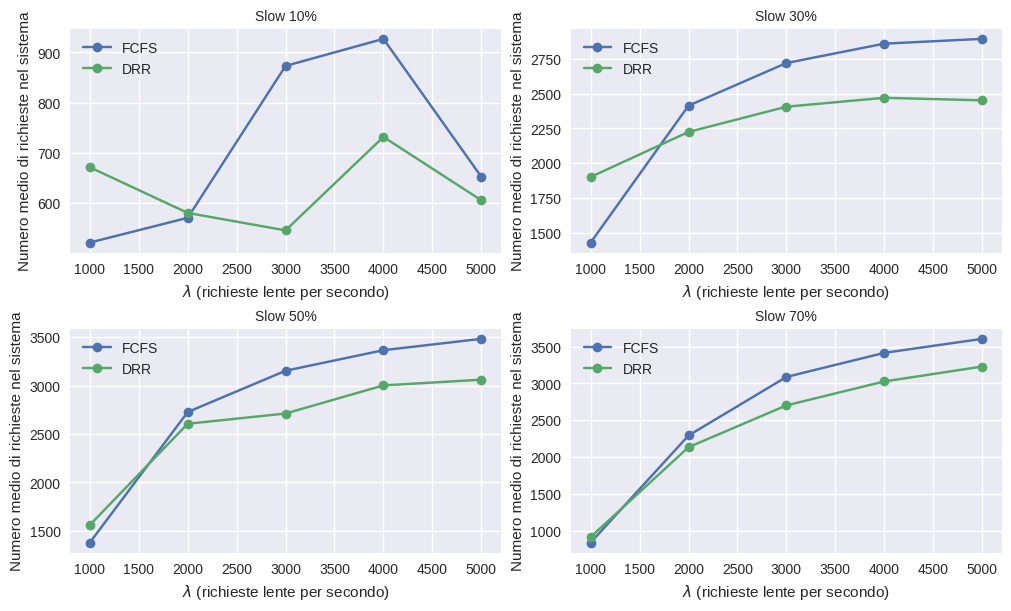
\includegraphics[width=\textwidth]{img/results/jobs.png}
  \caption{Andamento numero medio di richieste nel sistema.}
  \label{fig:jobs}
\end{figure}

\subsection{Utilizzazione CPU}
Dando priorità alle richieste veloci, la CPU spende meno tempo in media in attesa del completamento della richiesta lenta. Infatti, come mostrato in \cref{fig:cpu}, con l'algoritmo DRR, $\rho$ arriva fino al $70\%$; mentre, con FCFS raggiunge il $64\%$ solo con carico di richieste lente al $70\%$ con $\lambda=2000$. Si noti che in ipotesi di numero di richieste lente uguali a quelle veloci ($slow=50\%$), $\rho$ migliora del $30\%$.

\begin{figure}
  \centering
  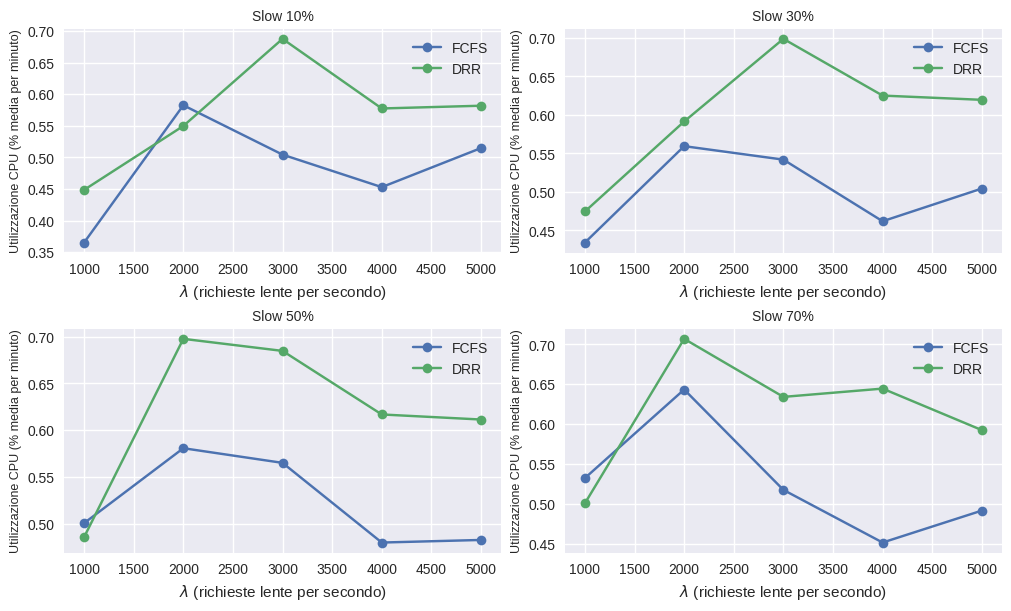
\includegraphics[width=\textwidth]{img/results/cpu.png}
  \caption{Andamento utilizzo processore.}
  \label{fig:cpu}
\end{figure}